\documentclass{article}
\usepackage[utf8]{inputenc}
\usepackage{float}
\usepackage{amsmath}
\usepackage{authblk}
 
\title{Emulation of a Biological Model Simulator}


\date{Dated: \today}

\author[,1]{Antoine Guiot \thanks{Email address: \texttt{antoine.guiot@supelec.fr}}}
\author[2]{Louis Philippe }
\author[3]{Eliott Tixier}
\author[,4]{Frederic Cogny}
 
\affil[1]{CentraleSupélec}
\affil[2]{Nova Discovery}
\affil[3]{Nova Discovery}
\affil[4]{Nova Discovery}





\usepackage{natbib}
\usepackage{graphicx}
\usepackage[a4paper, total={6in, 8.5in}]{geometry}
\begin{document}
\maketitle

\begin{abstract}
    This project presents two different approaches to speed up the resolution time of differential systems of equations. At first, a kriging approach has been studied. This provides good results but very limited mostly due to the long computation of this method. Then we implemented a more recent technique based on neural networks and long short term memory (LSTM) cells, once trained, this emulator might be better than the kriging-based emulator in terms of mean-square error (MSE). Even if these second results look good, our emulator remained biased. To fix this issue we tried to implement a multi-model-training method. This method presented in[3] reduced the bias of our emulator and significantly improved our MSE score. Although these results look really good, it is necessary to notice that multi training methods could be very expensive in computational time.
\end{abstract}
\newpage
\tableofcontents
\newpage

\section{Introduction}

This project has been proposed by Nova Discovery, a company working for the pharmaceutical industry. Nova Discovery's main work is focused on helping the drugs industry to develop and commercialize theirs medications. To do so, Nova Discovery's bio-modelers work on the modelization of complex interactions between drugs' active ingredients and patients. The idea is to describe the evolution of patients parameters during the time after taking a medication. 

\begin{figure}[h!]
\centering
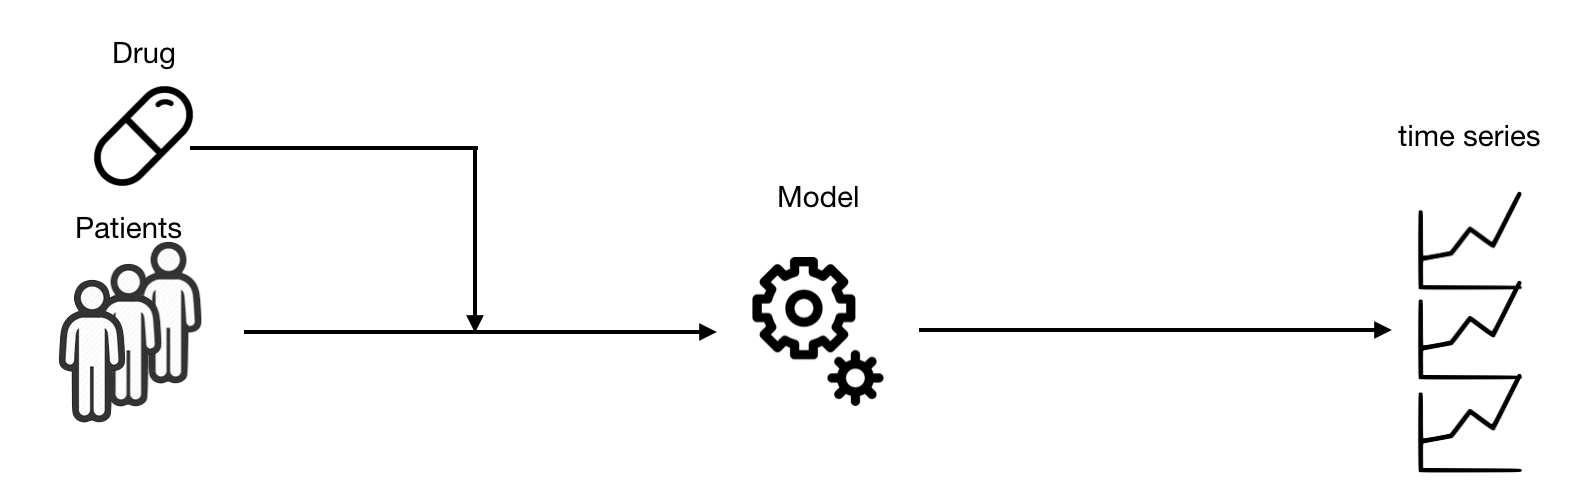
\includegraphics[scale=0.4]{image/introduction_fig.png}
\caption{In silico prediction of drug efficacy}
\label{fig:Drug efficacy prediction}
\end{figure}

A more mathematical approach would be: 

- let  
$p$ patient parameters and $m$ drug parameters  

We want to model the evolution of $p$ as: 
\begin{equation}
    p(t) = f(p_0,m,t)
\end{equation}
\\
with $p_0$ patient parameters at time $t=0$    

$p(t) = \begin{pmatrix}
p_1(t)\\
p_2(t)\\
\vdots \\
p_n(t)\\
\end{pmatrix}$

and:

$m = \begin{pmatrix}
m_1\\
m_2\\
\vdots \\
m_k\\
\end{pmatrix}$

$f$  is the solution of a non-linear differential equations system. Depending on the complexity of the system, finding the solution $f $ using classical equation solving methods (such as Euler's method) could be very expensive in computation time. This long computation time could become a problem when many patient starting parameters or many drug parameters must be tested.  

\section{Model Emulator}
In this context, one solution could be the emulation of these complex systems of equations. 
The principle of an emulator is to approximate the model output with lower computation time.

The process to create an emulator could be done in three steps:

  \\
- Model output sampling  \\
- Training the emulator on the sampled set   \\
- Testing our accuracy on a test data set    \\


\begin{figure}[h!]
\centering
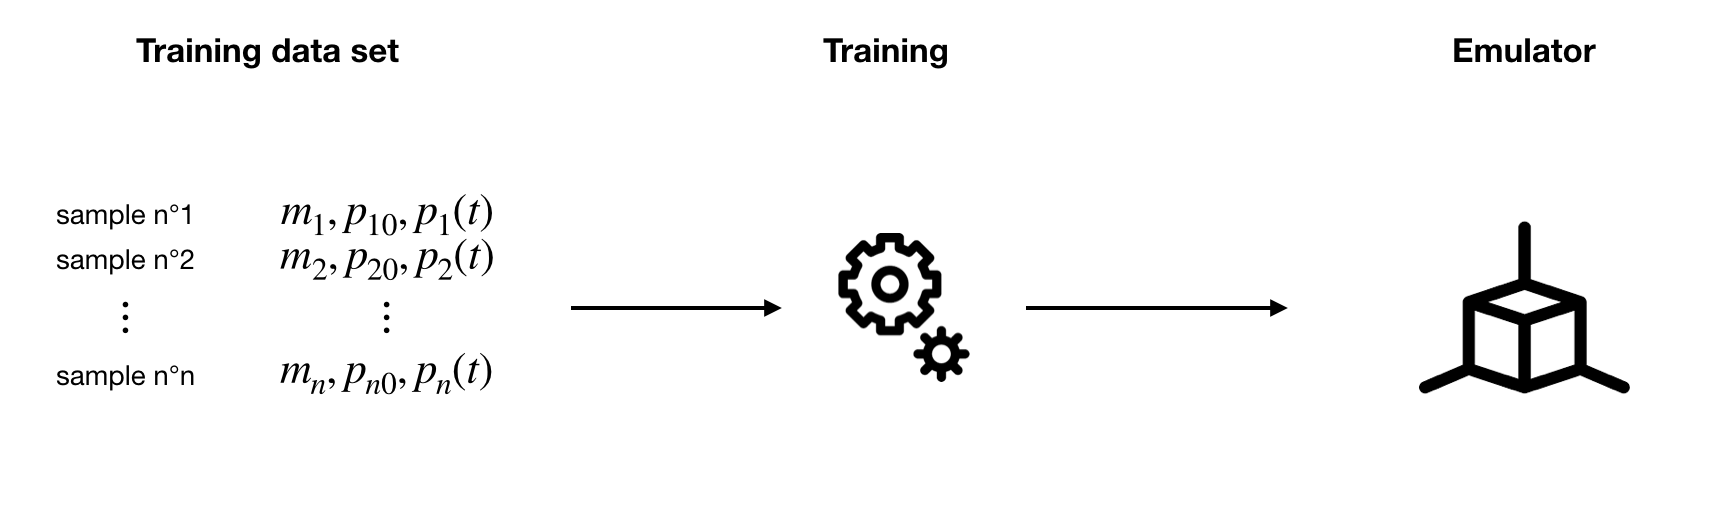
\includegraphics[scale=0.4]{image/emulator_creation.png}
\caption{Emulator training}
\label{fig: Emulator training}
\end{figure}

The creation of the emulator could be very expensive in terms of computation time. At first, the system of equations must be solved many times in order to create the training data set. Then training a machine learning model on this data, depending on the training method, can be long. But when this step is done, the emulator can provide an approximation of a solution for any input parameters in very small computation time.

\begin{figure}[H]
\centering
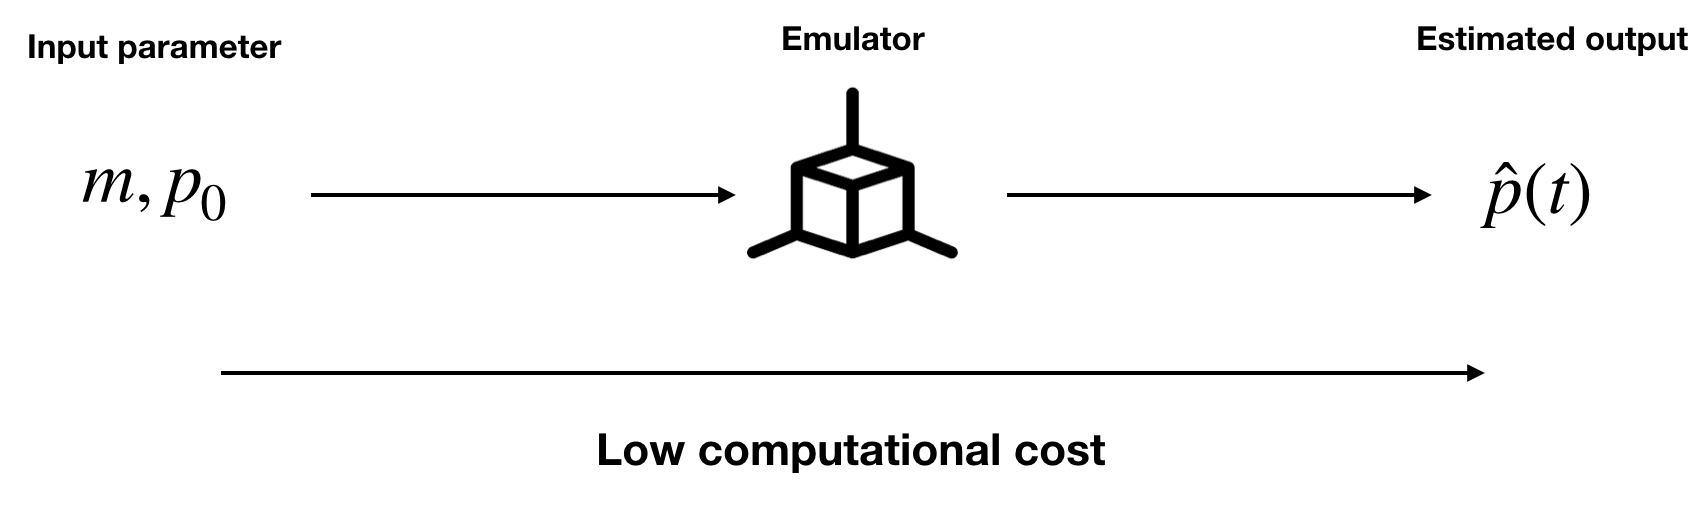
\includegraphics[scale=0.4]{image/emulator_after_training.png}
\caption{Emulator training}
\label{fig: Emulator estimation}
\end{figure}

\section{Simplified problem: Lotka-Voltera}

To focus our efforts on the quality of our emulator, we dealt with a very simple differential equations model:
Defined as:

\\
\begin{equation}
   \frac{dx}{dt}= \alpha x -\beta xy
\end{equation}

\begin{equation}
\frac{dy}{dt}= \delta xy - \gamma y
\end{equation}



with $p_0 =$ $\begin{pmatrix} x_0\\ y_0\\ \end{pmatrix}$
and  
$m = \begin{pmatrix} \alpha \\ \beta \\ \delta \\ \gamma \end{pmatrix}$
\\

With $y = y_{predator}$ and $x = y_{prey}$

The model must simulate two times series ( $y_{prey}(t)$ and $y_{predator}(t)$ knowing six input parameters ($\alpha$, $\beta$, $\gamma$, $\delta$, $y_{prey}(0)$, $y_{predator}(0)$)
\begin{figure}[H]
\centering
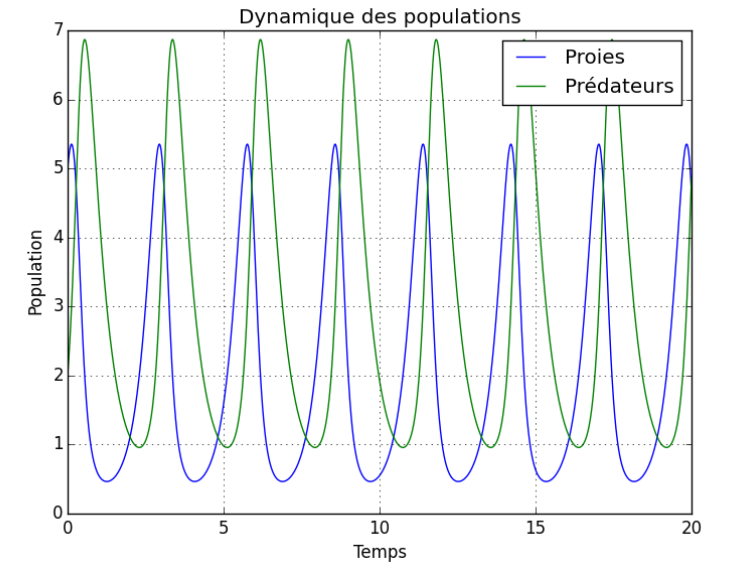
\includegraphics[scale=0.6]{image/lotka-volterra.png}
\caption{Lotka-Voltera example}
\label{fig: Lotka-Voltera example}
\end{figure}

\section{Sampling method}

As explained in fig : \ref{fig: Emulator training}, to train our emulator, a sampled training data set is needed. Knowing that sampling this training data set could be very expensive, we would like to obtain a good approximation with a minimum training set size. 


\subsection{Uniform sampling}
The first naive approach could be a uniform sampling of the parameter space. Here we have six parameters, let us say we want to sample each parameter in $[0;1]$, if we want to have a good representation of our parameter space we can take a 0.1 step for each parameter. 
This would result in a  training set of size $10^6$ samples.


\subsection{LHS sampling}
 Of course, the sampling of $10^6$ points can't be done in a reasonable time. We will use a Latin hyper-cube sampling which can provide a good representation of the parameter space with very few points. The method performs the sampling by ensuring that each sample is positioned in a space $\Omega$ of dimension $d$ (six in our case)  as the only sample in each hyperplane of dimension $d-1$ aligned with the coordinates which define its position.
The figure below shows an example of this sampling with $d =2$:

\begin{figure}[H]
\centering
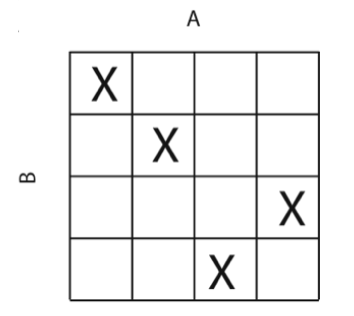
\includegraphics[scale=0.6]{image/lhs_d_2.png}
\caption{Latin hyper-cube sampling with $d =2$}
\label{fig: latin hypercube sampling example}
\end{figure}

In the next sections, we will see the impact of the training set size on the accuracy of our emulator. Hopefully, we should have a good precision with less than $10^6$ points.

\section{Kriging}
In current literature, many papers dealing with the emulation of differential systems of equations tackle the problem using Gaussian processes and kriging (such as \cite{ml_using_gaussian_process}). In this first approach, we implemented this method and then bench-marked different kernels and training methods 

\subsection{Theory}

We want to approximate $\hat{f}(x_{n+1})$ as a function of previous sampled points.   \\
Let $x_i$ $i \in [0;n]$ the set of sampled points  \\
Let $K = Cov(f(x_i),f(x_j))_{i,j \in [0;n]}$   \\
We suppose that $K_{n+1} = Cov(f(x_i), \hat{f}(x_{n+1}))_{i \in [0;n]}$ is known   \\ 
We approximate $\hat{f}$ as
\begin{equation}
    \hat{f}(x_{n+1}) = \sum_i \lambda_i f(x_i) 
\end{equation}
   \\
and compute 

\begin{equation}
  \lambda = K^{-1} K_{n+1}    
\end{equation}{}
 

We can define different kernels for our co-variance matrix $K$   \\ 
  \\ 
$K_{RBF}(\theta, x_i, x_j) = e^{-\frac{1}{2}d(\frac{x_i}{l},\frac{x_j}{l})^2}$
  \\
$K_{Matern}(\theta, x_i, x_j) =\sigma^2 e^{-\gammad(\frac{x_i}{l},\frac{x_j}{l})^2}$
  \\ 
$K_{Quadratic}(\theta, x_i, x_j) = (1+ \frac{d(x_i,x_j)^2}{2\alpha l^2})^{-\alpha}$


\subsection{Results}
In this section presents results of the kriging approach. 
\subsubsection{Mean square error (MSE)}

The MSE is computed as follow:  \\
Let $N$ the number of samples in the testing data set.  \\
Let $n$ the number of points in a time series.   
 \\  
 \\  
 \begin{equation}
     MSE_{prey} = \sum_{j=0}^{N} \sum_{i=0}^{n} (f_{prey_j}(t_i) - \hat{f}_{prey_j}(t_i))^2 
 \end{equation}
 
\\  
\begin{equation}
    MSE_{predator} = \sum_{j=0}^{N} \sum_{i=0}^{n} (f_{predator_j}(t_i) - \hat{f}_{predator_j}(t_i))^2 
\end{equation}


\begin{figure}[H]
\centering
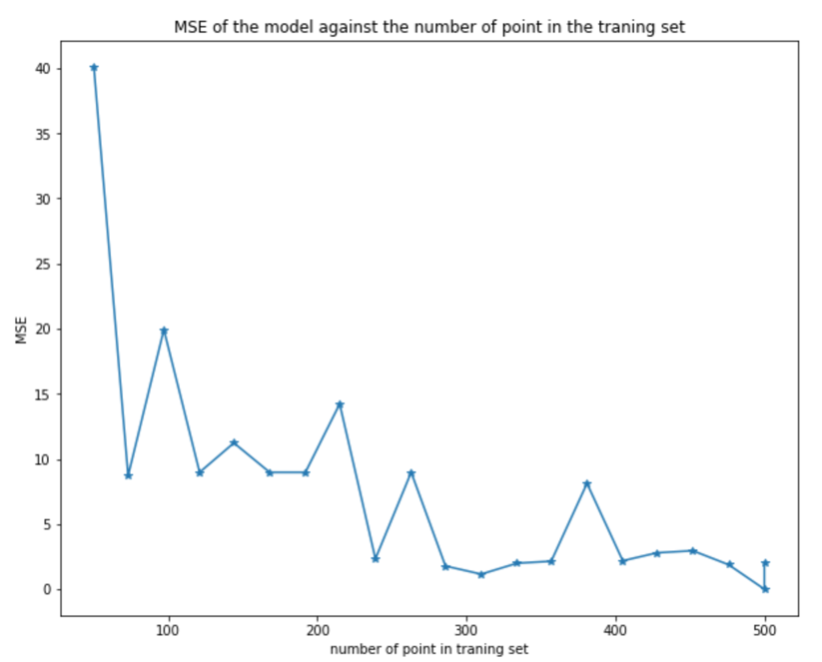
\includegraphics[scale=0.6]{image/mse_kriging.png}
\caption{Mean square error of prey time series as function of the number of points in the training data set}
\label{fig: kriging MSE}
\end{figure}
As expected, the MSE is a decreasing function of the training set size. The best case is obtained with 500 samples (MSE = 2.43). The major problem of this approach is the training time which explodes when the training set size is more than 500. That's why we didn't explore this approach with a very large training data set. The fig \ref{fig: training_time_explosion} shows this computation time explosion. 

\begin{figure}[H]
\centering
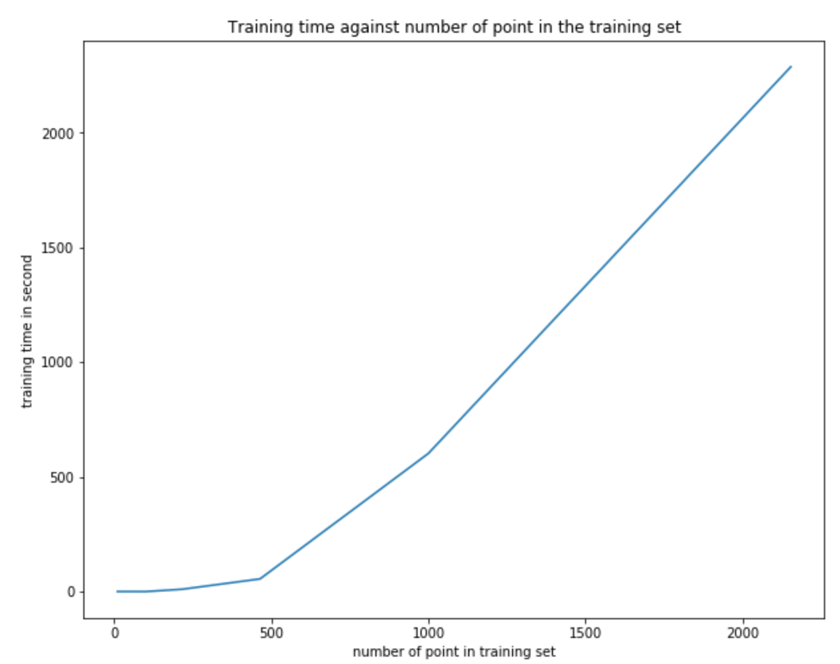
\includegraphics[scale=0.6]{image/kriging_time_explosion.png}
\caption{Training time in seconds as a function of the data set size. We can observe an explosion of the training time when training set size is up to 500 points.}
\label{fig: training_time_explosion}
\end{figure}
\section{Neural network based approach}

In this approach, we tackle the problem using more recent methods. We based our model on the research paper from Shangying Wang, Kai Fan & al (2019) \cite{emulation_using_NN}. The main idea is to approximate our output time series using a neural network-based method with LSTM cells.

\subsection{LSTM cells}

LSTM (Long short-term memory) cells have been first presented in 1997 by Sepp Hochreiter and Jürgen Schmidhuber \cite{Long_short_term_memory}

LSTM architecture is composed of a cell (the memory part of the LSTM unit) and three "regulators", usually called gates, of the flow of information inside the LSTM unit: an input gate, an output gate and a forget gate. 

Intuitively, the cell is responsible for keeping track of the dependencies between the elements in the input sequence. The input gate controls the extent to which a new value flows into the cell, the forget gate controls the extent to which a value remains in the cell and the output gate controls the extent to which the value in the cell is used to compute the output activation of the LSTM unit.

\begin{figure}[H]
\centering
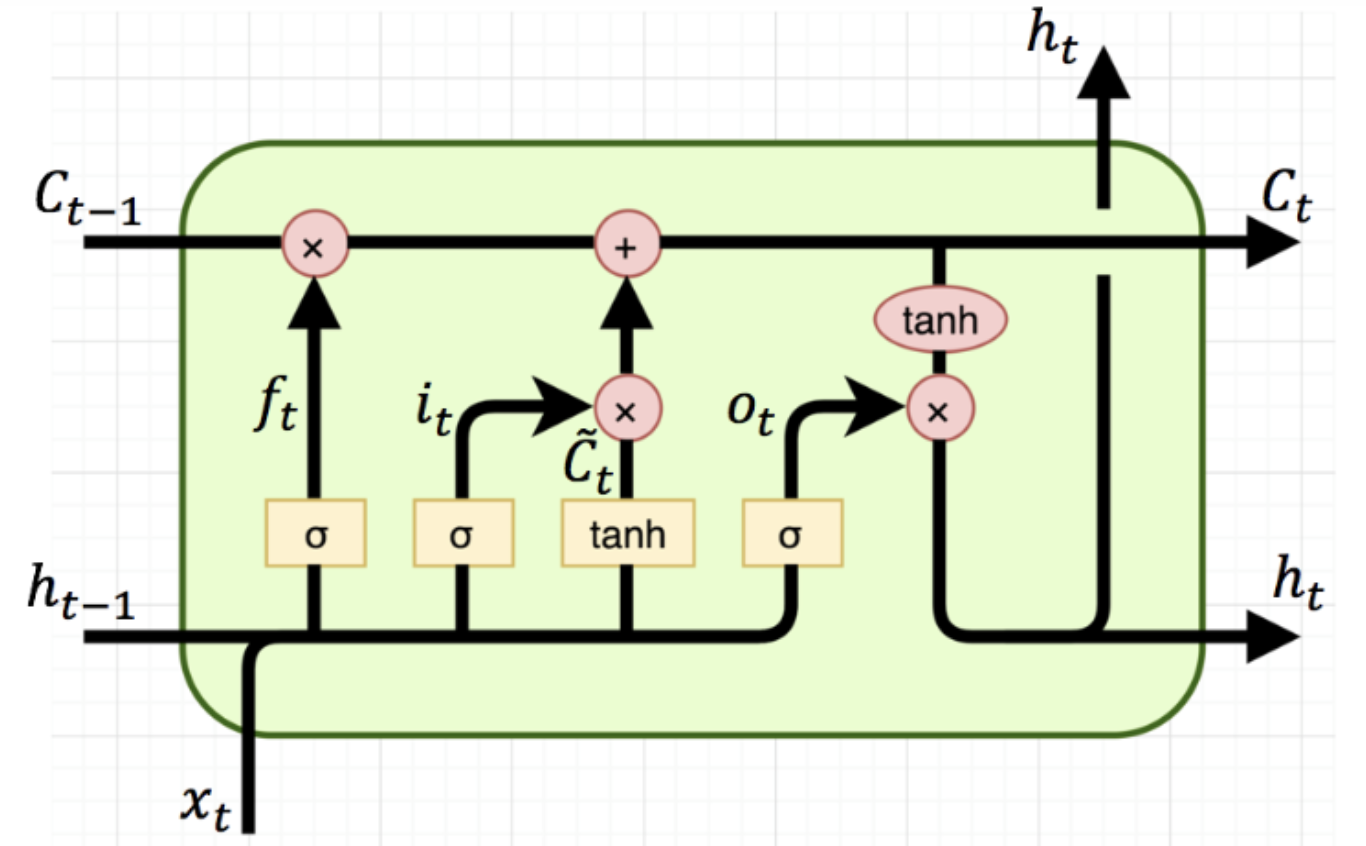
\includegraphics[scale=0.4]{image/lstm_cell.png}
\caption{LSTM cell architecture,}
\label{fig: lstm_cell}
\end{figure}
\\  
  
$x_t$ : input vector to the LSTM unit \\
$f_t$ : forget gate's activation vector\\
$i_t$ : input/update gate's activation vector\\
$o_t$ : output gate's activation vector\\
$h_t$ : hidden state vector also known as output vector of the LSTM unit\\
$\tilde{c}_t$ : cell input activation vector\\
$c_t $ : cell state vector\\



\subsection{Preprocessing}
This article precises that LSTM network would be efficient to forecast times series scaled between 0 and 1. So we decomposed the problem into two sub-problems: the first task is the prediction of the re-scaled time series (predict a series of values between 0 and 1) and the second task is the prediction of the minimum and maximum values of the time series. 
  \\  
  \\  
  \begin{equation}
      \Tilde{f}_{prey}(t) = \frac{f_{prey}(t)-f_{prey_{min}}}{f_{prey_{max}}-f_{prey_{min}}}
  \end{equation}

  \\  
 \begin{equation}
     \Tilde{f}_{predator}(t) = \frac{f_{predator}(t)-f_{predator_{min}}}{f_{predator_{max}}-f_{predator_{min}}}
 \end{equation}


\begin{figure}[H]
\centering
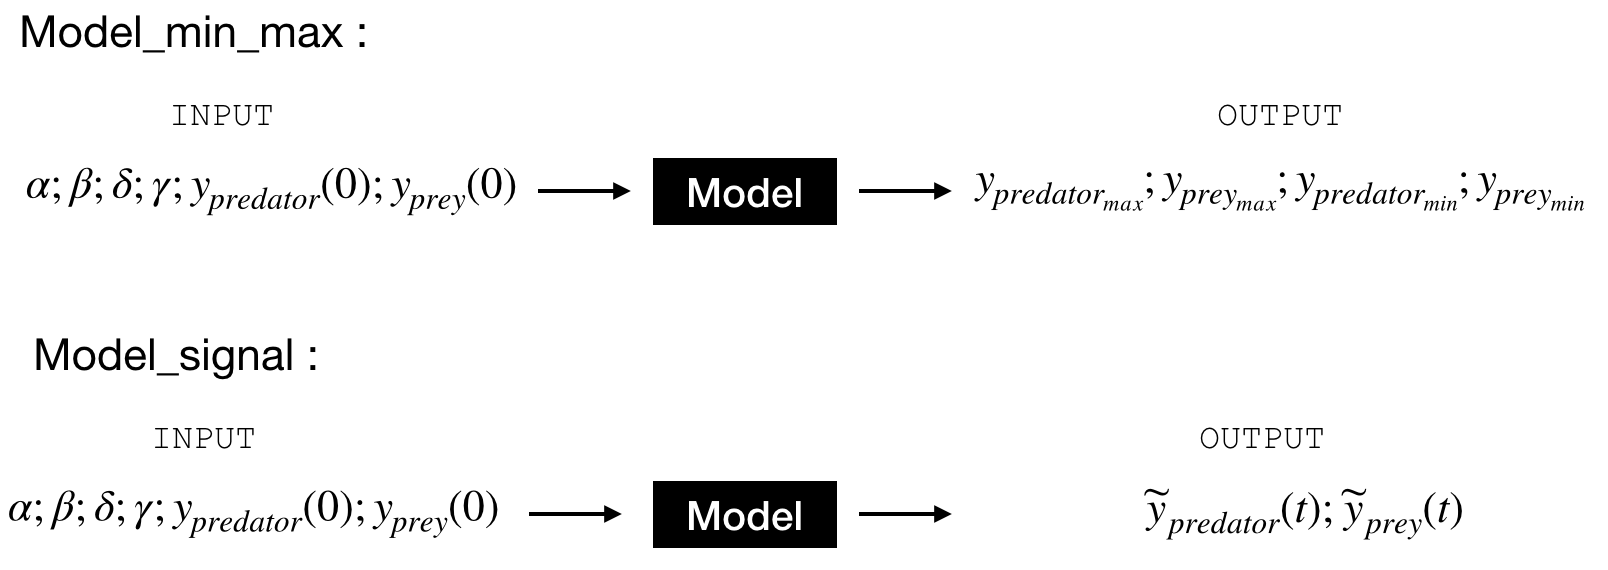
\includegraphics[scale=0.4]{image/models_explanation.png}
\caption{Two different tasks for NN approach}
\label{fig: Two models}
\end{figure}


\subsection{Models}
\subsubsection{Min Max model }

The first task is processed by a succession of dense fully connected layers. Parameters (number of layers, number weight per layer) has been tuned with an empirical approach. An efficient tuning of these hyperparameters could be a good idea for future work on this subject.  


\begin{figure}[H]
\centering
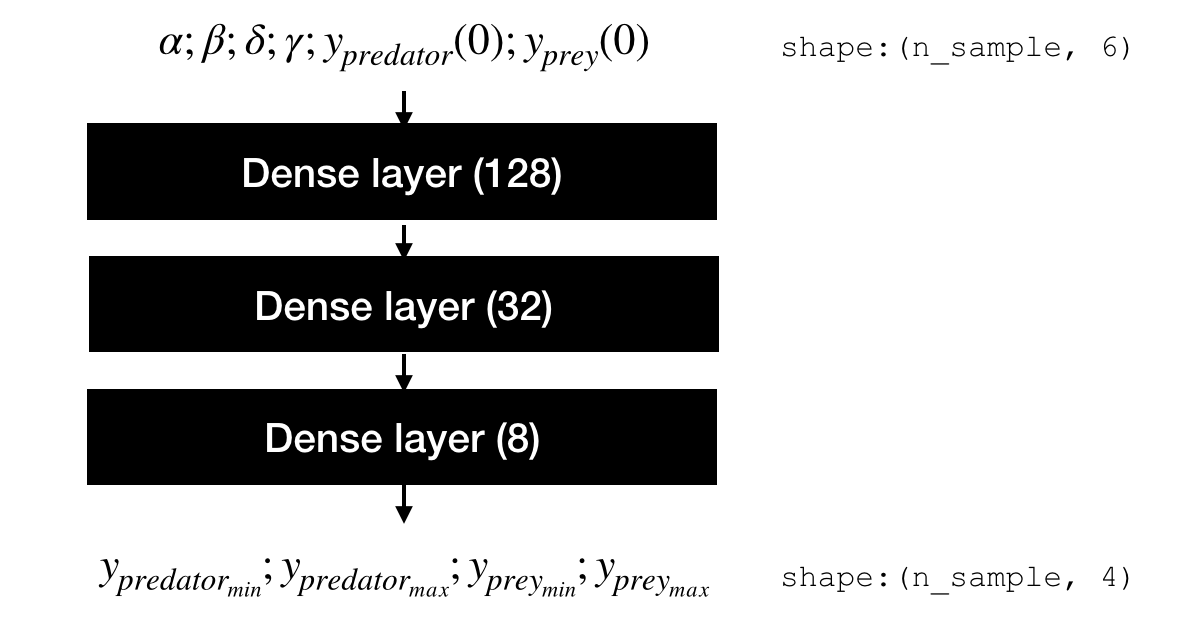
\includegraphics[scale=0.4]{image/min_max_model.png}
\caption{Min max model architecture}
\label{fig: Two models}
\end{figure}

\subsubsection{Time series model}

The second task is done by a dense layer followed by an LSTM layer. As same as before, parameters such as the number of neurons in each layer as been tuned empirically. The figure below shows the architecture of the model.   

\begin{figure}[H]
\centering
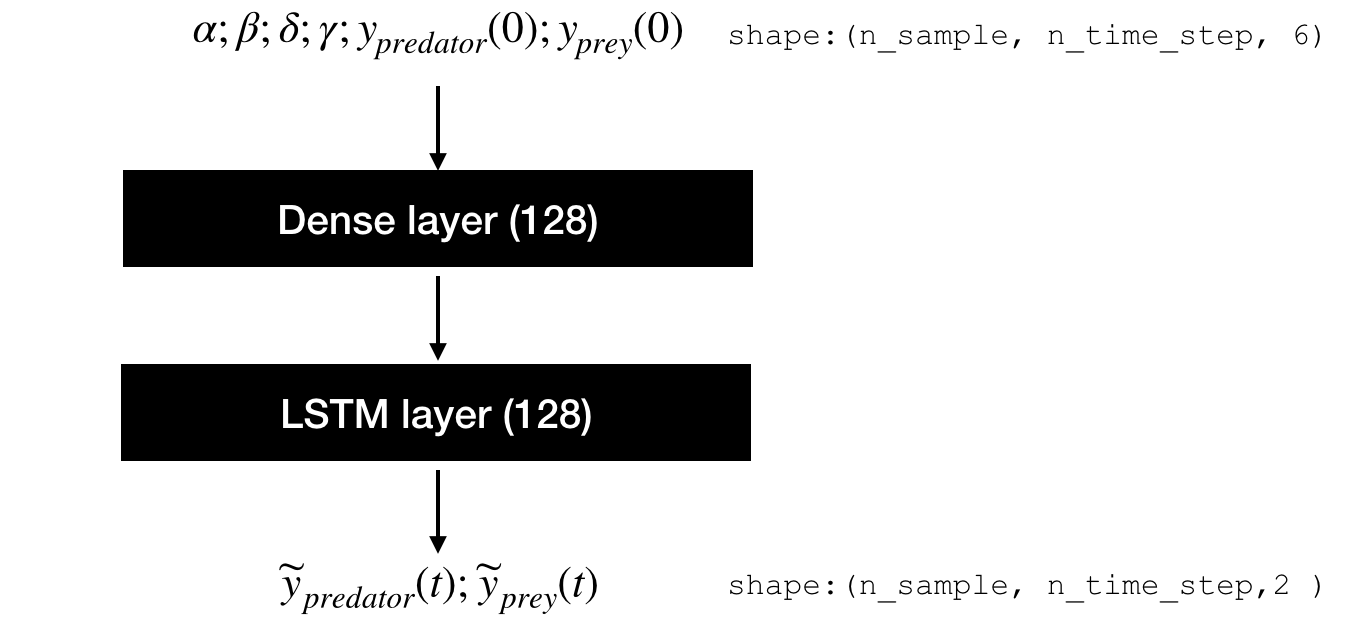
\includegraphics[scale=0.4]{image/signal_model.png}
\caption{Signal model architecture}
\label{fig: Signal model}
\end{figure}


\subsection{Results}

In this section, we detail our results with this model. We created a testing sample data set of size 500 points (random sampling with all parameters between 0 and 1). This testing set is used to compute the mean square error (MSE) of the model. We would like to see the impact of the training data set size on the MSE of the testing data set.

\subsubsection{Mean square error (MSE)}

\begin{figure}[H]
\centering
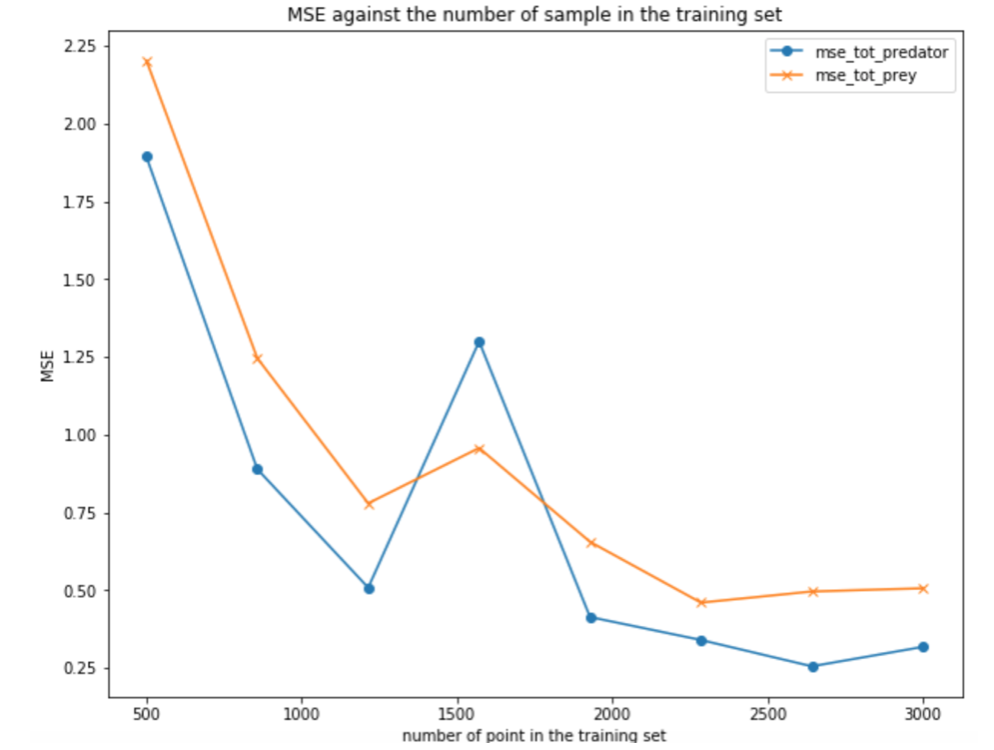
\includegraphics[scale=0.5]{image/mse_NN.png}
\caption{Influence of the training set size on the MSE of the NN based model computed on a 500-points testing data-set}
\label{fig: Signal model}
\end{figure}

The figure above presents the MSE of two time series. As expected, the MSE decreases when the number of points in the training set increases. It seems to be stabilizing when the training set size is up to 2000 points.  \\
This figure brings a good decision tool to decide which sampling set size will provide an efficient emulator. 

\subsubsection{Residuals}

Now we take a look at our emulator residuals.  \\

We compute residuals as follow: \\
For $i \in [0; n]$, $j \in [0, N]$ 
\begin{equation}
    R_{i+jn} = f_{prey_j}(t_i)- \hat{f}_{prey_j}(t_i)
\end{equation}
  \\  
If $\hat{f}$ is a consistent estimator of $f$. Residuals of $\hat{f}$ should be normal distributed around 0. 





\begin{figure}[H]
\centering
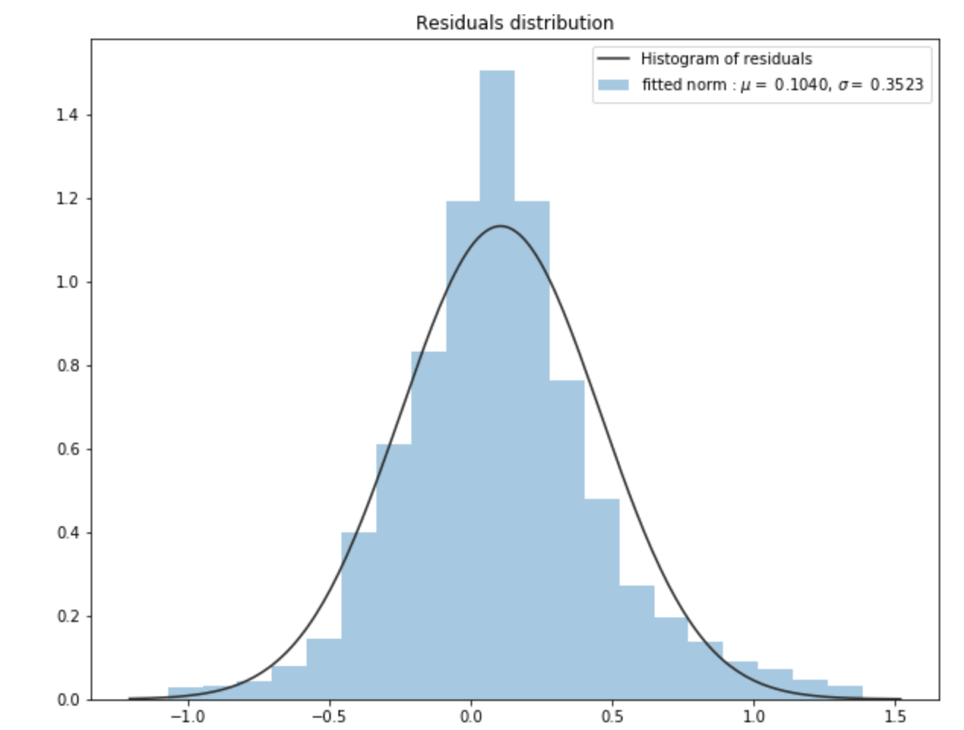
\includegraphics[scale=0.5]{image/distrib_residuals_NN.png}
\caption{Residuals distribution of $\hat{f}$ trained on a 3000 points data set. }
\label{fig: Signal model}
\end{figure}

As we can see in the figure above, our estimator seems to be biased. Even if we increase the number of points in the training set the mean of the distribution remains far from zero.


\begin{figure}[H]
\centering
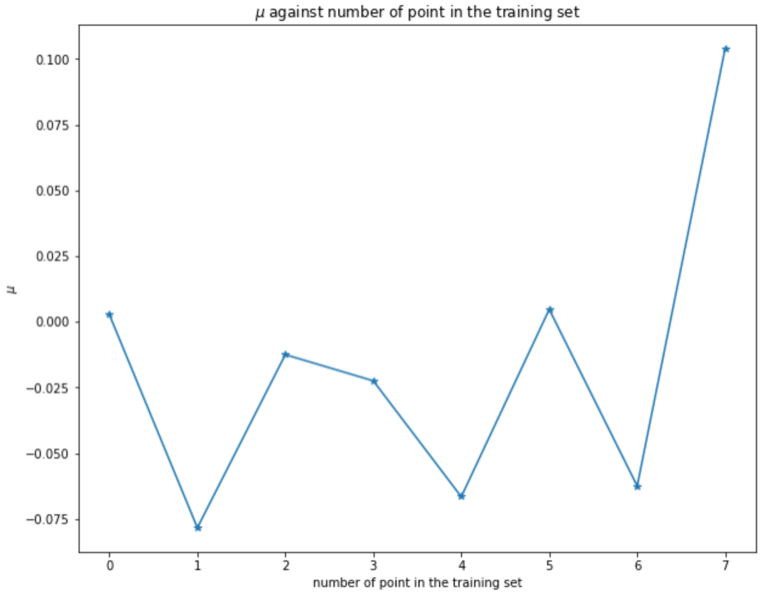
\includegraphics[scale=0.6]{image/mu_against_nb_pts.png}
\caption{Bias values vs number of point in training set }
\label{fig: Signal model}
\end{figure}

The fig \ref{fig: sigma reduction} below shows us the variance reduction when the training set size increases, meaning that our estimator becomes better with a larger training set (but still biased). 

\begin{figure}[H]
\centering
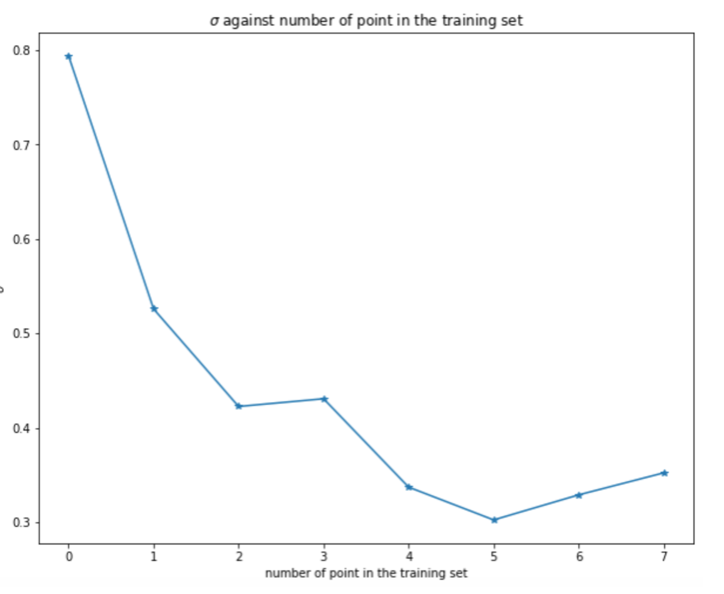
\includegraphics[scale=0.6]{image/sigma_reduction_signal.png}
\caption{Sigma reduction when training set size increases}
\label{fig: sigma reduction}
\end{figure}


In section 8 we will discuss a method to reduce bias in estimators. 

\subsubsection{Results on some time series}

\begin{figure}[H]
\centering
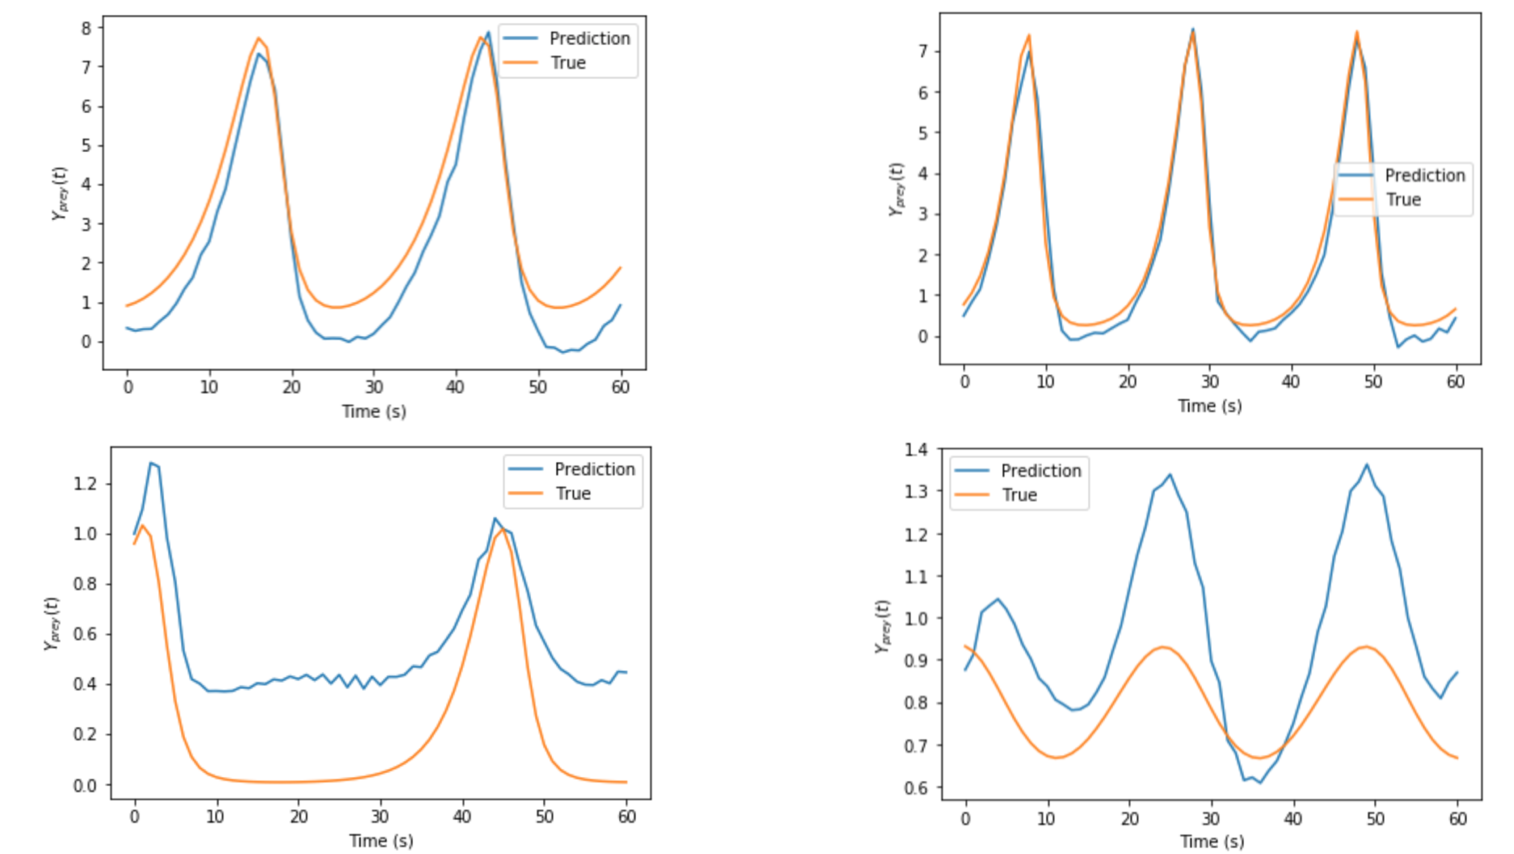
\includegraphics[scale=0.4]{image/some_time_series_signal.png}
\caption{Results for some time series (trained on 3000 points)}
\label{fig: some time series}
\end{figure}

\subsection{Limits}
According to the presented results, our emulator seems to be quite accurate and, with some limitations (bias, variance), could be useful.  But, in this previous work, we limited the parameters spaces to a very small subspace of $R_+^6$. The figure below presents an experiment where all parameters have been sampled (using LHS sampling) in $[0;10]$. 

\begin{figure}[H]
\centering
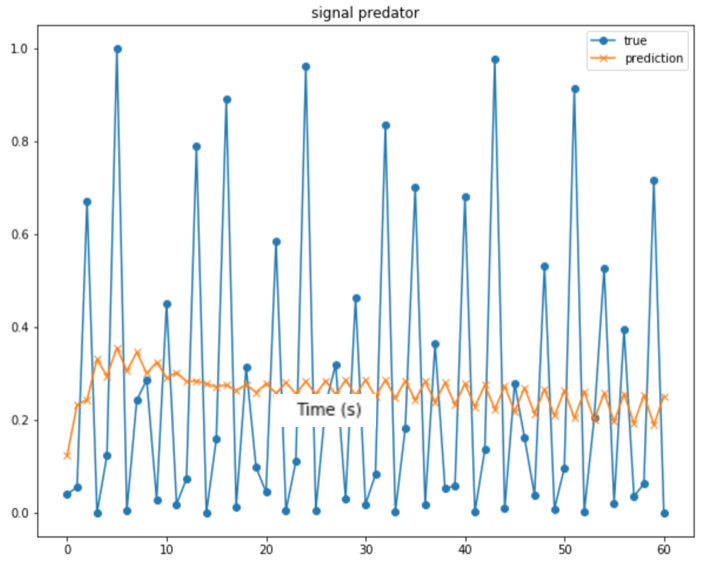
\includegraphics[scale=0.6]{image/limitation_time_series.png}
\caption{Emulator results for parameters sampled in $[0;10]^6$. Blue: true time series. Green: predicted time series.)}
\label{fig: some time series}
\end{figure}

It is important to notice that the true time series has very important variations and, with very small time-sampling, looks discontinuous. It appears that our model cannot deal with this type of discontinuous time series. Two different solutions can be found to avoid this problem. \\
- Avoid this type of time series in the training set by reducing the parameters space to a subspace with smooth time series. (Could not work if we want an emulator working in a large parameter space containing discontinuous times series.)  \\
- Reduce the time-sampling step (ie. increase the number of points in each time series). This solution could lead to an explosion of the training time (the number of weights in the model would explode). Moreover, when the number of weights in the model increases, we should increase the training set size. Knowing that sampling time series could be very expensive in computation time: it would become impossible to build this emulator in a reasonable time (see introduction)).  




\section{Scores}

When the system of equations has been solved (with classical equation solver or emulator), the next step is to compute "scores". Scores are computed from the solved time series, and represent useful values for Nova Discovery. In this section, we explore the idea of training a model to solve scores instead of time series.   \\

Scores are computed as follow: \\

We compare the value of $f(t_i)$ with reference values $\alpha$ and $\beta$ : \\
if $f(t_i) > \alpha$  $\to$ $S(t_i) = 1$\\
if $f(t_i) < \beta$  $\to$ $S(t_i) = 0$ \\ 
elif $f(t_i) \in [\beta ; \alpha] $ $\to $ $S(t_i) = g(f(t_i))$ 


\begin{figure}[H]
\centering
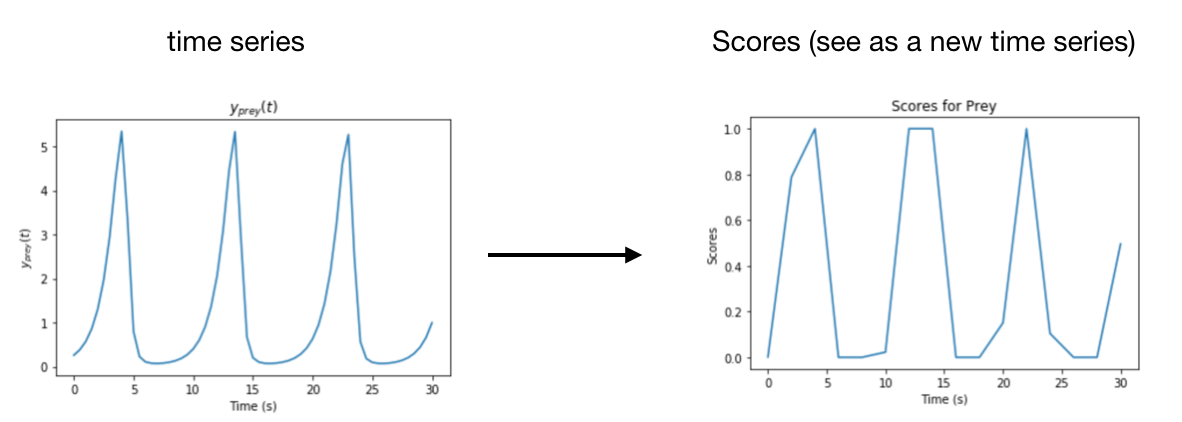
\includegraphics[scale=0.6]{image/time_serie_vs_scores.png}
\caption{From time series to scores}
\label{fig: time_ series to score}
\end{figure}

\subsection{Model}
Scores can be seen as a new time series with a lower number of points. Moreover, all points are scaled between 0 and 1. It results in a simplified problem with less dimensions and with all values between 0 and 1(So it is not necessary to rescale time series and create a min-max model) (see section 6.3). The emulator has the same architecture as the times series model from part 6.3.2 

\begin{figure}[H]
\centering
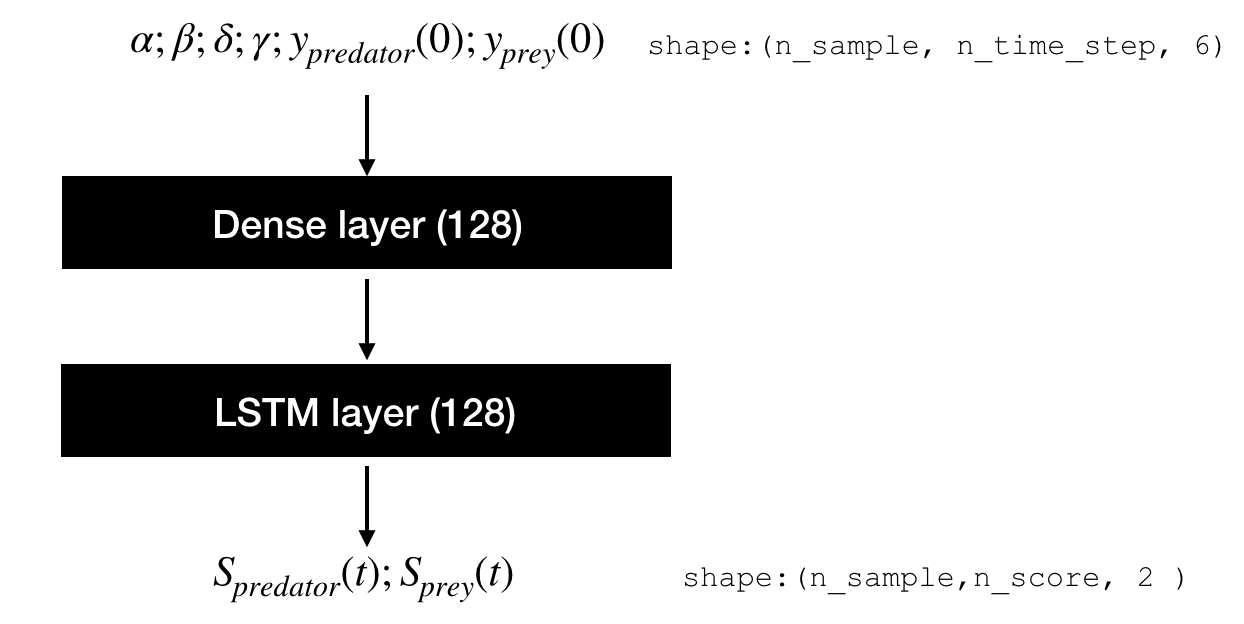
\includegraphics[scale=0.4]{image/scores_archite.png}
\caption{Architecture of scores emulator}
\label{fig: scores emulator}
\end{figure}

Same as before, we trained this emulator on a latin hypercube sampling subset of the parameter space. 

\subsection{Results}

\subsubsection{MSE}
\begin{figure}[H]
\centering
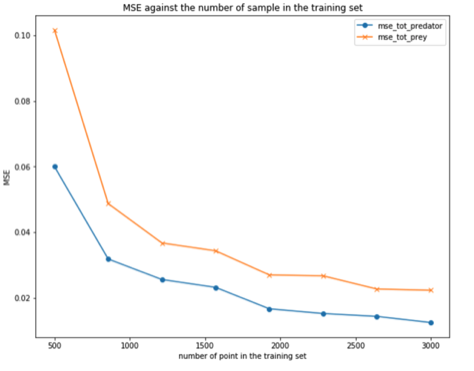
\includegraphics[scale=0.5]{image/MSE_score.png}
\caption{MSE of scores time series vs number of points in the training set}
\label{fig: scores MSE}
\end{figure}

As we can see on the figure below, the MSE for the score model seems to be much better than the one for the classic time series model. 
\\  
\\  
- MSE Scores best case : 0.02 \\
\\
- MSE Time series best case 0.3 \\ 

\begin{figure}[H]
\centering
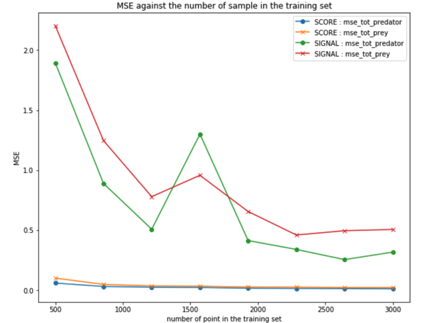
\includegraphics[scale=0.6]{image/mse_comparison.png}
\caption{This figure compare the MSE for the classical approach (named as SIGNAL : ) and the MSE for the scoring approach (named as SCORE)}
\label{fig: Comparison_MSE}
\end{figure}

\subsubsection{Residuals}


This section presents some results on score-model residuals. Same as before we will study variance and bias of this emulator.   


\begin{figure}[H]
\centering
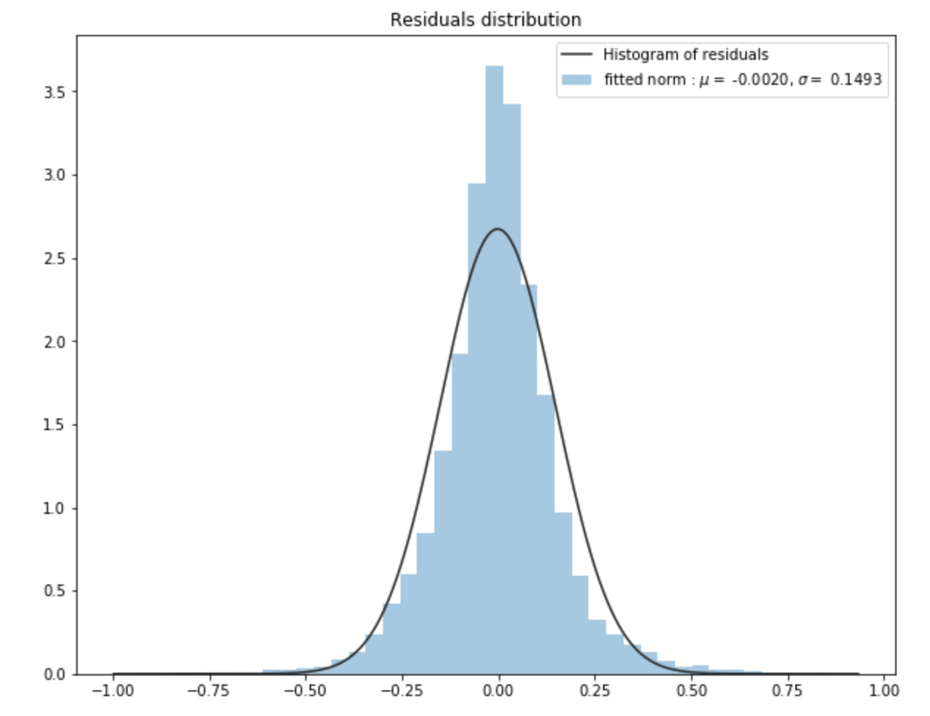
\includegraphics[scale=0.5]{image/score_distribution.png}
\caption{Distribution of residuals for scores emulator, trained on a 3000 samples data set}
\label{fig: scrore distrib}
\end{figure}  

$\sigma$ = 0.1493 ;
$\mu$ = 0.002 \\

The figure below presents the variance of $\mu$ when the number of points in the training data set increases. Same as before, the value seems to be distributed around zero, following a random distribution. But in this case, the value of $\mu$ is much closer to zero.

\begin{figure}[H]
\centering
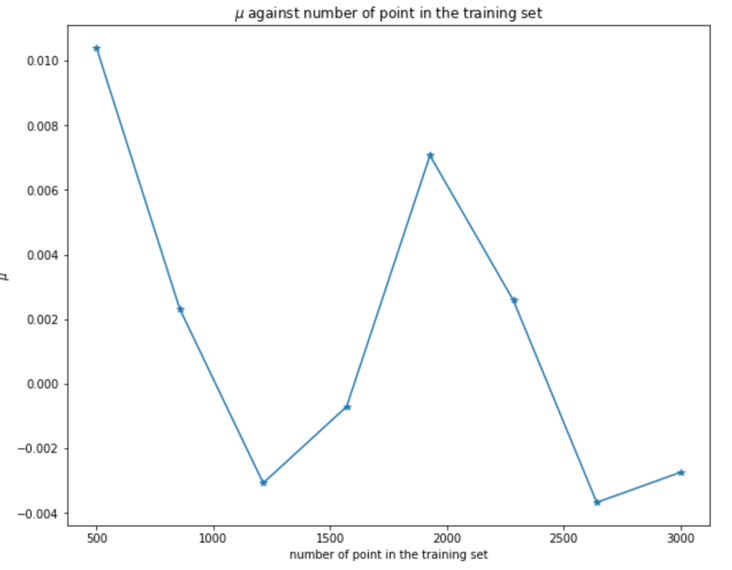
\includegraphics[scale=0.6]{image/mu_variation_score.png}
\caption{Residuals mean variation against the number of points in training set is increasing}
\label{fig: scrore mean variation}
\end{figure}

Next figure shows the variance reduction for this approach. As shown in fig \ref{fig: variance comparison} the variance for this approach always remains below the variance for the previous approach.   

\begin{figure}[H]
\centering
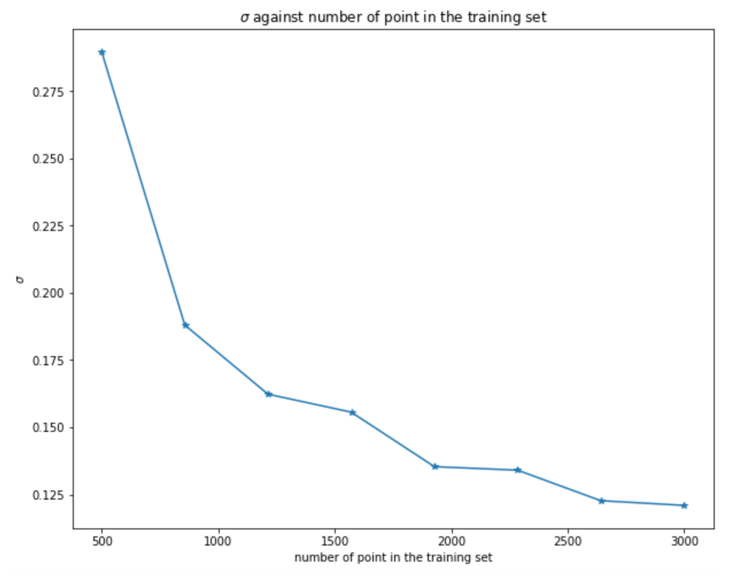
\includegraphics[scale=0.6]{image/sigma_reduction_score.png}
\caption{Sigma reduction for score emulator}
\label{fig: scrore mean variation}
\end{figure}


\begin{figure}[H]
\centering
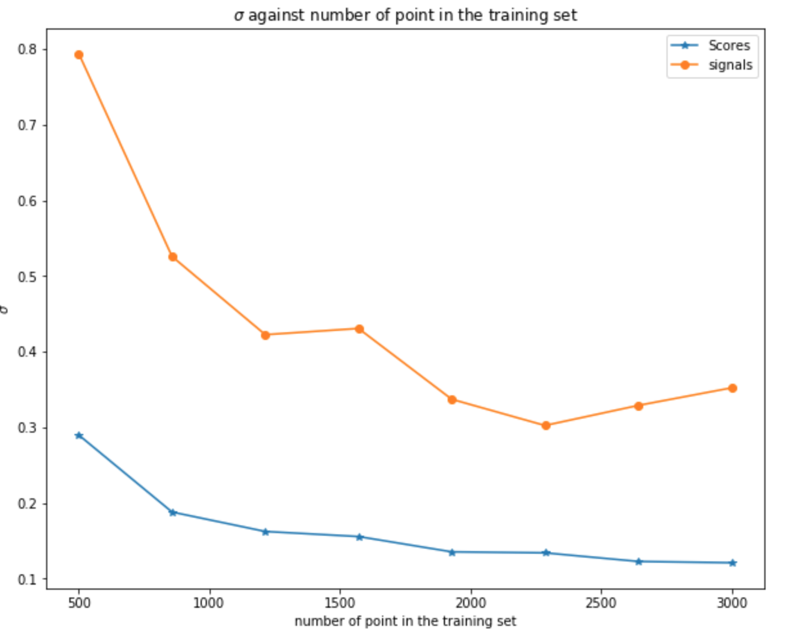
\includegraphics[scale=0.55]{image/variance_reduction_comparison.png}
\caption{Sigma comparison (Score emulator : Blue, Time series emulator : Green)}
\label{fig: variance comparison}
\end{figure}


\subsubsection{Results on some scores}

\begin{figure}[H]
\centering
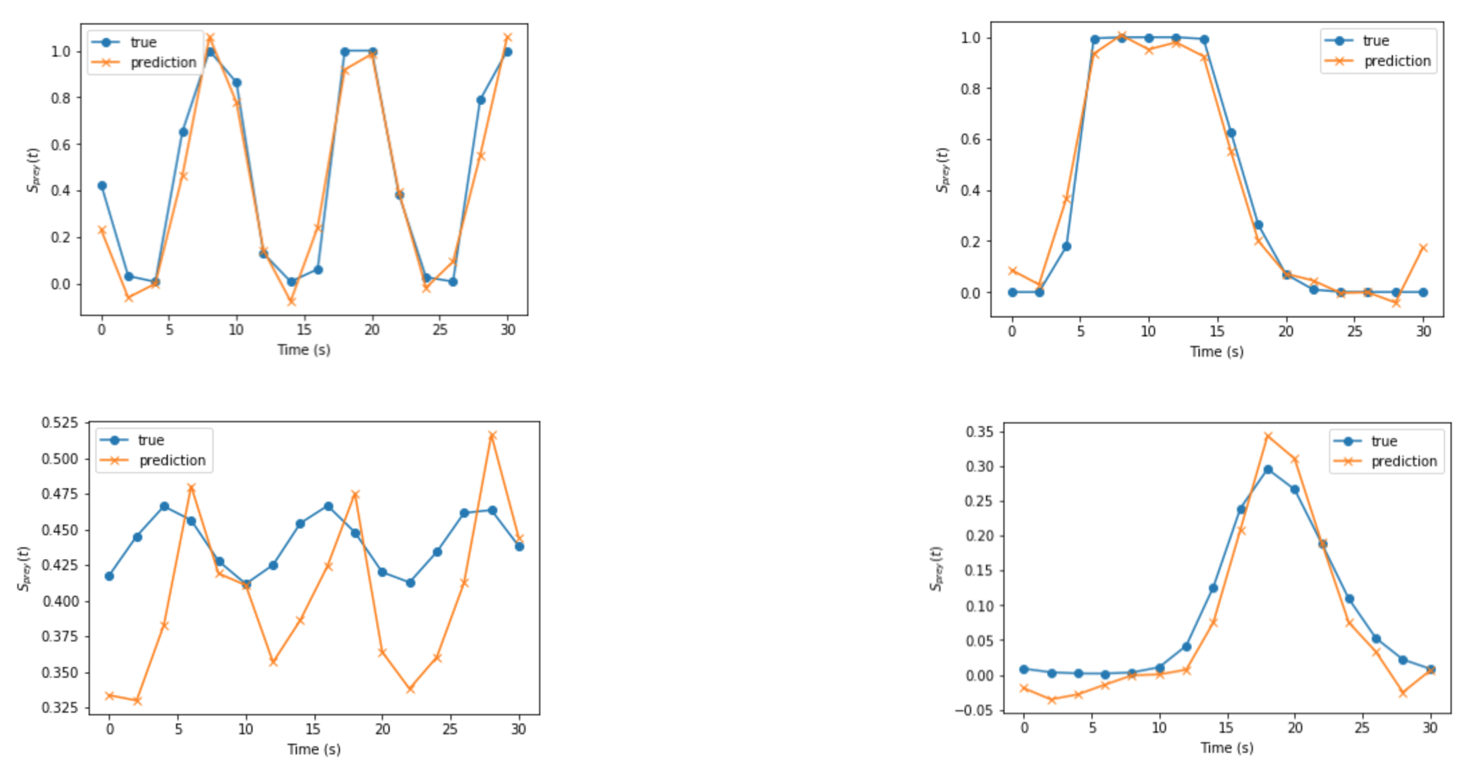
\includegraphics[scale=0.4]{image/examples_on_scores.png}
\caption{Results for some time series (trained on 3000 points)}
\label{fig: variance comparison}
\end{figure}


\section{Reducing bias}
This section presents a useful idea to reduce bias in emulators. As presented in section 6, the time series emulator implemented with a neural network remains biased even if the number of points in the training data set becomes very large. To fix this issue, Shangying Wang, Kai Fan & al  \cite{emulation_using_NN} propose to train different models.  The idea is that for each model, model weights are randomly-initialized, then after training: all models can be considered as different. We compute the output of the multi-model as the mean of all models outputs. (See fig \ref{fig: multi_model})
$\forall$ $i$
\begin{equation}
    \hat{f}(t_i)= \frac{1}{N} \sum^N_{j=1} \hat{f}_j(t_i)
\end{equation}
 \\ 
With N the number of models.

More complex approaches could be implemented: 

\\ - Each model is trained with different hyper-parameters

\\ - Each model is trained on a different part of the parameter space.

\\ - Each model is trained on a different data set size 

Hopefully, each model will provide a biased emulator with random bias: distributed around zero. Then when computing the final emulator as the mean of each emulator: the final bias will be reduced.    

Results from the last technique are presented below. Future work on this subject could be focused on a benchmark of all multi-model training techniques. 

\begin{figure}[H]
\centering
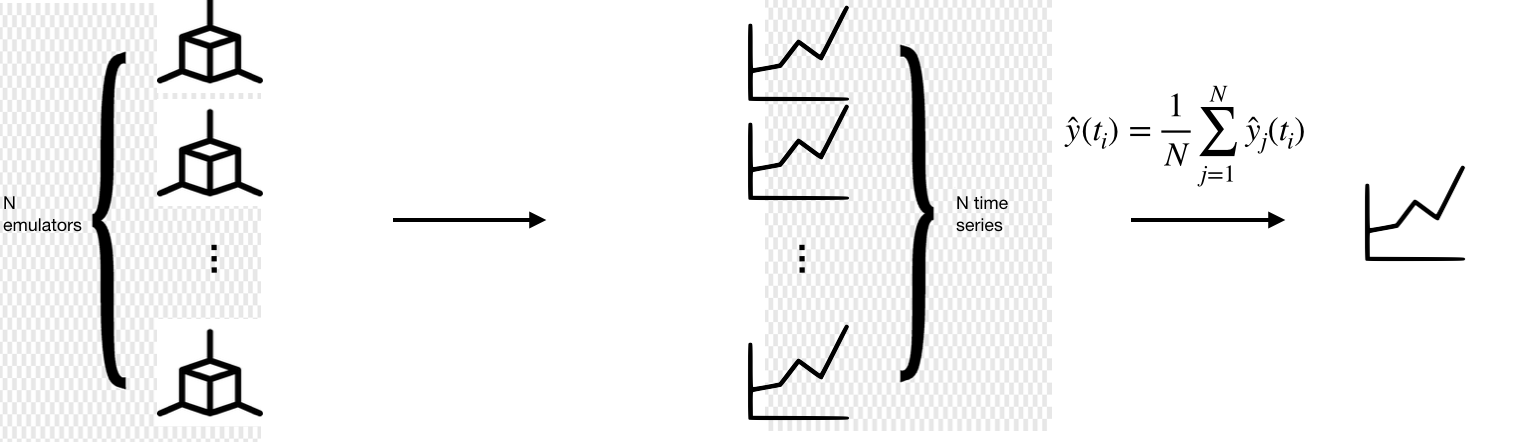
\includegraphics[scale=0.4]{image/multi_model.png}
\caption{Multi model training architecture for bias reduction}
\label{fig: multi_model}
\end{figure}

\subsection{Results}
\begin{figure}[H]
\centering
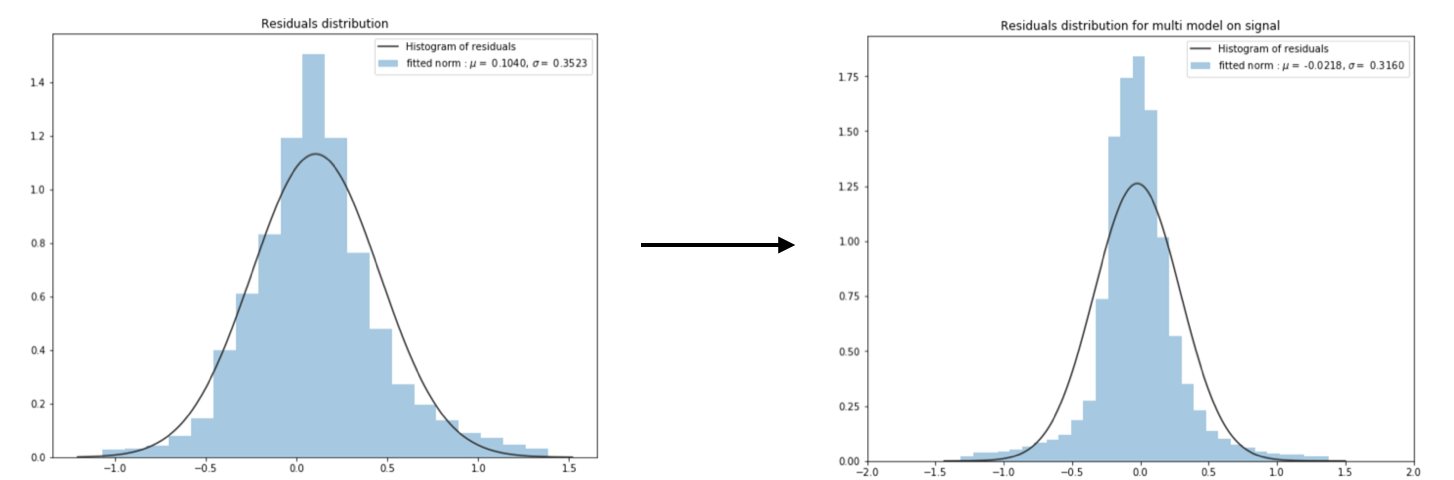
\includegraphics[scale=0.5]{image/multi-model-signal.png}
\caption{Influence of multi-model training on residuals distribution for time series emulator. Left: residuals distribution without multi training ($\mu = 0.104 , \sigma = 0.35$. Right: residuals distribution after multi model training (8 models trained on [ 500,  857, 1214, 1571, 1928, 2285, 2642, 3000] points) ($\mu = 0.0218$, $\sigma =0.031$) }
\label{fig: influance of multi model training on mu}
\end{figure}

The fig \ref{fig: influance of multi model training on mu} shows that multi-model training has an important impact on bias reduction. Then the fig \ref{fig: influance of multi model training on mse} presents the impact of multi-model training on the MSE of time series. It can be seen that the impact on MSE looks interesting (goes from 0.255 for the best case to 0.016). This first iteration of multi-model training provides good results for this emulator and it would be interesting to see how do other methods improve our accuracy (MSE).


\begin{figure}[H]
\centering
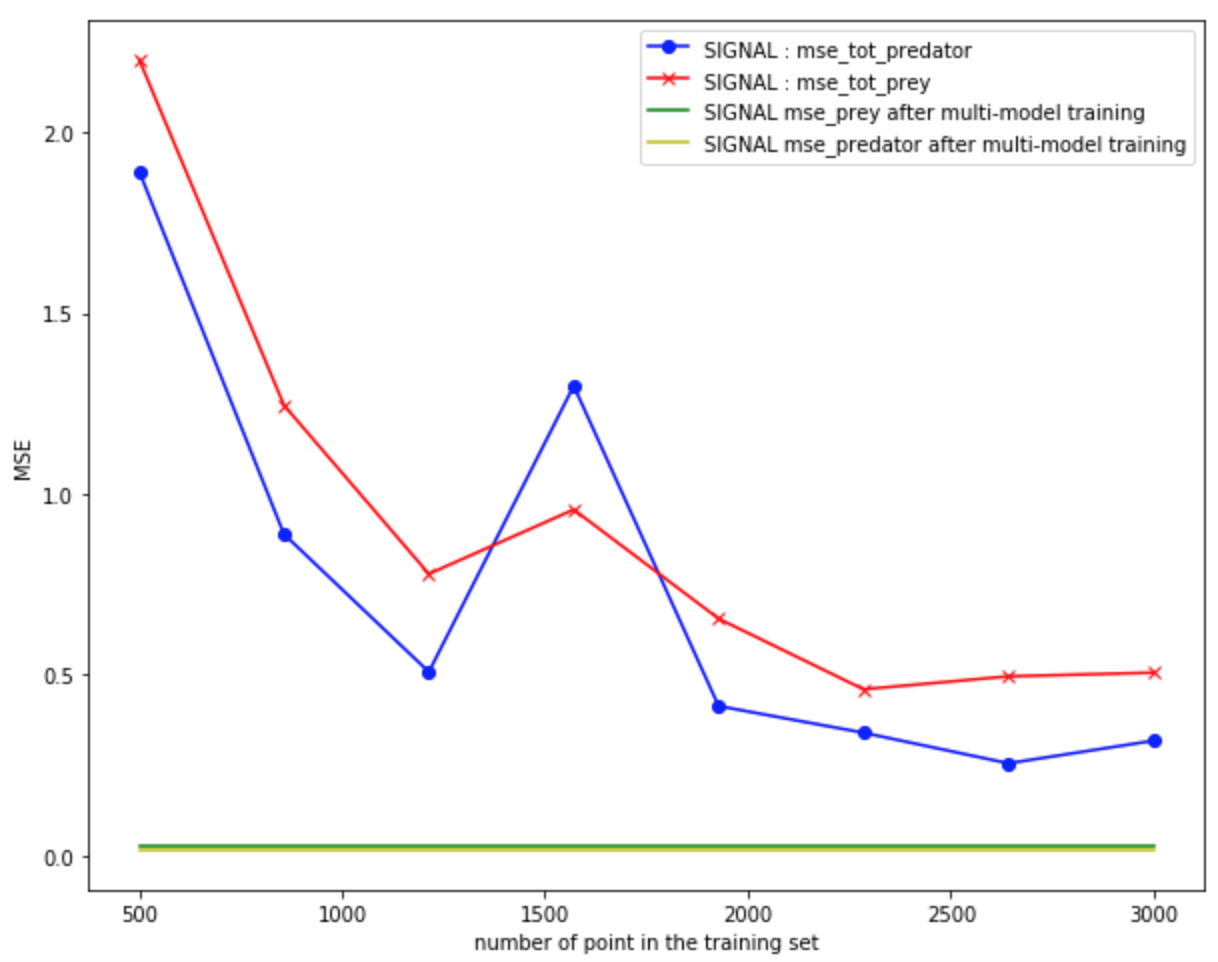
\includegraphics[scale=0.5]{image/mse_reduction.png}
\caption{MSE reduction. Red: MSE reduction of prey time series when the training set size increases. Blue: MSE reduction of predator time series when the training set size increases.  Green: prey time series MSE for the final model, computed as the average of 8 models trained on different data sets. Yellow: predator time series MSE for the final model computed as the average of 8 models trained on different data sets.}
\label{fig: influance of multi model training on mse}
\end{figure}


\section{Conclusion}

The project goal was about being able to reproduce a differential equations-based model behaviour without solving the system of equations. At the end of this project, we partially achieved this goal for a simple system of equations. According to the mean square error, the variance and the bias: the emulators based on a neural network approach seem to provide better results, especially when coupled with a multi training. 

We have demonstrated some limitations of our approaches:\\
- Emulators must be limited to a subspace of the parameters space.
\\
- Emulators are more efficient if time series are scaled in $[0;1]$ 
\\
- A large training set is needed (3000 samples in our example)
\\
An interesting future work on this project should focus on "How do these emulators perform on more complex models?"  Moreover, we just tried a very simple method for multi training. A next step could also be focused on implementing more complex multi-training algorithms. 





\newpage
\bibliographystyle{plain}
\bibliography{references}

\end{document}


